\documentclass[11pt]{article}
\pagestyle{empty}
%\usepackage[latin1]{inputenc}
\usepackage[utf8]{inputenc}
\usepackage{a4wide}
\usepackage{amsmath}
\usepackage{amssymb}
\usepackage{amsthm}
\usepackage{german}
\usepackage{multirow,array}
\usepackage{hyperref}
 \usepackage{graphicx}
%\usepackage{ipe}
%\input{thmstyle-ger}

\parindent0mm
\sloppy

% Basic data
\newcommand{\VORLESUNG}{Induktive Statistik für Soziologinnen und Soziologen}
\newcommand{\STAFF}{Mariana Nold}
\newcommand{\ASSIGNMENT}{2}
\newcommand{\HANDOUT}{Montag, den 13. November   2017}
\newcommand{\DELIVER}{keine Abgabe, wird in der Übung besprochen}
\newcommand{\PRACTICAL}[1]{\marginpar{\tiny {\bf Aufgabe \\ abgeben!} #1}}
\newcommand{\FAUFTRAG}[1]{\marginpar{\tiny {\bf selbst entdeckendes Verstehen} #1}}
\newcommand{\titel}{Grundlagen des statistischen Testens}
\newcommand{\startwert}{3}

% Arbitrary packages and settings

\newcommand{\N}{\mathbb{N}}
\newcommand{\floor}[1]{\lfloor{#1}\rfloor}
\newcommand{\ceil}[1]{\lceil{#1}\rceil}
\newcommand{\half}[1]{\frac{#1}{2}}
\newcommand{\punkte}[1]{{\small{ }(#1 Punkte)}}
\newcommand{\punkt}[1]{{\small{ }(#1 Punkt)}}

\newcommand{\aufgabe}[1]{\item{\bf #1}}
\newcommand{\hinweis}{{\em Hinweis}}

\begin{document}
% Document title

\begin{center}
\ASSIGNMENT{}. Übungsblatt vom \HANDOUT{} zur Vorlesung 
\vspace*{0.5cm}

{\Large \VORLESUNG{}}
%\PRACTICAL{}
(\STAFF{}) 


\vspace*{0.5cm}
{\textbf{Thema:} \titel{}\\}
\vspace*{0.2cm}

{\small Abgabe: \DELIVER{}}
\vspace*{1cm}
\end{center}

Wichtige Definitionen:
\begin{enumerate}
\item{Inferenzschluss}
\item{gerichtete Hypothese}
\item{ungerichtete Hypothese}
\item{Fehler 1. Art ($\alpha$-Fehler)}
\item{Fehler 2. Art ($\beta$-Fehler)}
\item{Teststatistik des Zwei-Stichproben t-Test}
\item{Ablauf des Zwei-Stichproben t-Test}
\item{kritischer Wert und Ablehnbereich}
\item{p-Wert}
%\item{Binäre Variable und  Bernoulliverteilung}
%\item{Binomialverteilung}
\end{enumerate}
\vspace{2cm}
\begin{enumerate}\addtocounter{enumi}{\startwert}





\aufgabe{Der $\chi^{2}$-Test:  Statusverlustangst und relative Deprivation im Thüringen-Monitor $2015$}\\
(vgl. Aufgabe 18, des 5. Übungsblattes im letzten Semester.)\\
Leseempfehlung: LWLG: S. 212-218\\

Schlagen Sie Ihre Formelsammlung auf S. 51 auf. Dort finden Sie unter $8.5.1$ den \\
$\chi^{2}$-Unabhängigkeitstest. Das Wort Prüfgröße ist ein Synonym für Teststatistik.
Die Teststatistik des $\chi^{2}$-Unabhängigkeitstest ist mit dem $\chi^{2}$-Koeffizienten
identisch.
Die Prüfgröße lautet

$$
\chi^{2}= \sum_{j=1}^{m} 
\sum_{k=1}^{q} \frac{\big(h(x_{j},y_{k})-h_{e}(x_{j},y_{k})\big)^2}{h_{e}(x_{j},y_{k})}.
$$

\begin{itemize}
\item{Es ist $h(x_{j},y_{k})$ die Häufigkeit mit der die Kombination $(x_{j},y_{k})$
beobachtet wurde, $j \in \{1, 2\}$ und $k \in \{1, 2\}.$}
\item{Es ist $h_{e}(x_{j},y_{k})$ die bei Unabhängigkeit erwartete Häufigkeit 
der  Kombination $(x_{j},y_{k}).$}
\end{itemize}
 	


\vspace{0.5cm}
% Augabe mit der Notation von LM lösen und die äquivalente Notation angeben
Zur Erinnerung an Definitionen aus  der Vorlesung (im letzten Semester):

Die Frage nach der Statusverlustangst: ``Es macht mir Sorgen, durch die gesellschaftliche Entwicklung immer mehr auf die Verliererseite
 des Lebens zu geraten.''
 \begin{itemize}
   \item {Die Antwortkategorien: ``lehne ab,'' ``stimme zu''}
    \item {Im Datensatz: ``lehne ab = nein'' ($y_{1}$), ``stimme zu = ja'' ($y_{2}$)}
  \end{itemize} 
  Die Frage zur Deprivation: ``Im Vergleich dazu, wie andere hier in Deutschland leben: 
   Glauben Sie, dass Sie Ihren gerechten Anteil erhalten, 
   mehr als Ihren gerechten Anteil, etwas weniger oder sehr viel weniger?''
   \begin{itemize} 
   \item{Die Antwortkategorien: ``erhalte sehr viel weniger,'' ``erhalte etwas weniger,''  ``erhalte gerechten Anteil,''         
  ``erhalte mehr als gerechten Anteil,''  ``weiß nicht,'' ``keine Angabe''}
  \item{Im Datensatz:
    \begin{description}
    
     \item {
       \[
     \text{$x_{1}:$ ``erhalte weniger''}=\left\{\begin{array}{ll} \text{``erhalte sehr viel weniger,''} \\
         \text{``erhalte etwas weniger''}\end{array}\right. 
  \]
     }
      \item {
       \[
     \text{$x_{2}:$ ``erhalte genug''}=\left\{\begin{array}{ll} \text{``erhalte gerechten Anteil,''} \\
         \text{``erhalte mehr als gerechten Anteil''}\end{array}\right. 
  \]
     }
     %\item {(``erhalte gerechten Anteil,'' ``erhalte mehr als gerechten Anteil'')= ``erhalte genug,''}
    
    \end{description}
      }
 \end{itemize}

Im Thüringen-Monitor 2015 haben $940$ Personen sowohl die Frage nach der 
Statusverlustangst als auch nach der Deprivation beantwortet. Die anderen $70$ Personen haben mit ``weiß nicht'' oder ``keine Angabe''
geantwortet oder die Antwort vollständig verweigert. Die  Vierfeldertafel \ref{depri_angst} zeigt die bivariaten Häufigkeiten
der $940$ Personen.

%        erhalte.weniger erhalte.genug
%   nein             289           362
%   ja               214            75

  \begin{table}[ht]
\centering
\caption{Bivariate Häufigkeit: Statusverlustangst $Y$ und Deprivation $X$}



\begin{center}
\begin{tabular}{|c|c|c|}
	\hline %   
             & erhalte weniger   & erhalte genug  \\ \hline
        nein & $289$  & $362$                  \\ \hline
          ja & $214$  & $75$        \\ \hline
\end{tabular}
\end{center}
\label{depri_angst}
\end{table}
Lösen Sie die folgenden Aufgaben mit Hilfe von  \texttt{STATA 14:}
\begin{enumerate}
\item{Lesen Sie die beobachtete Häufigkeit $h(x_{1},y_{2})$ aus Tabelle \ref{depri_angst}
und interpretieren Sie diese Häufigkeit.}
 \item {Lesen Sie mit dem Befehl \texttt{. use ``monitor\_15.dta'', clear} den Datensatz ein und erstellen  Sie die Vierfeldertafel \ref{depri_angst}.}
 \item{Geben Sie den Befehlt \texttt{. tab2 Angst Deprivation, chi2} in das Command-Window ein
 und erklären lesen Sie den Werte des $\chi^{2}$-Koeffizienten und das  ab.}
 \item{ Erklären Sie mit Bezug auf den $\chi^{2}$-Koeffizient warum hohe Werte
 der Teststatistik gegen eine Unabhängigkeit der beiden
 Merkmale $X$ und $Y$ sprechen.}
 \item{Erklären sie mit Bezug auf die angegeben $2 \times 2$ Kreuztabelle, was man unter einem Inferenzschluss versteht. }
 \item{Wir möchten nachweisen, dass die beiden Merkmale $X$ und $Y$ (stochastisch) abhängig sind, wie können entsprechend die Nullhypothese
 und die Forschungshypothese formuliert werden?}% FT S. 466
 \item{Was versteht man unter dem Signifikanzniveau bzw. der Irrtumswahrscheinlichkeit?}
 \item{Legen Sie das Signifikanzniveau fest (auf $5\%$) und suchen Sie im \texttt{STATA-output} des Befehls \texttt{. tab2 Angst Deprivation, chi2}
 nach dem p-Wert. Kann die Forschungshypothese nachgewiesen werden?}
 \item{Es lässt sich zeigen, dass der $\chi^{2}$-Koeffizient unter $H_{0}$ einer $\chi^{2}$-Verteilung mit einem Freiheitsgrad folgt. Diese ist in Abbildung
 \ref{abb1} dargestellt. Es ist auch der kritische Wert $k$ eingezeichnet. Der kritische Wert ist $3.84.$
 \begin{itemize}
 \item[i)]{Der  $\chi^{2}$-Koeffizient entspricht im  $\chi^{2}$-Test der Teststatistik. Vergleichen Sie den Wert der Teststatistik mit dem kritischen Wert 
 $k=3.84.$ }
 \item[ii)]{Schlagen Sie die Formelsammlung auf S. 62 auf. Wie können sie den kritischen Wert ablesen?}
 \item[iii)]{Markieren Sie den Ablehnbereich farbig in Abbildung  \ref{abb1} und malen Sie die Fläche zwischen  Ablehnbereich und Dichtkurve aus. Wie hoch ist der Anteil der
 ausgemalten Fläche an der Fläche unter der Dichterkurve. }
 \item[iv)]{Quantifizieren Sie die Unsicherheit des Inferenzschlusses indem Sie Auskunft über den $\alpha$- und $\beta$-Fehler geben.}
 \end{itemize}
 }
\end{enumerate}
 \begin{figure}[ht]
 	\centering
 	      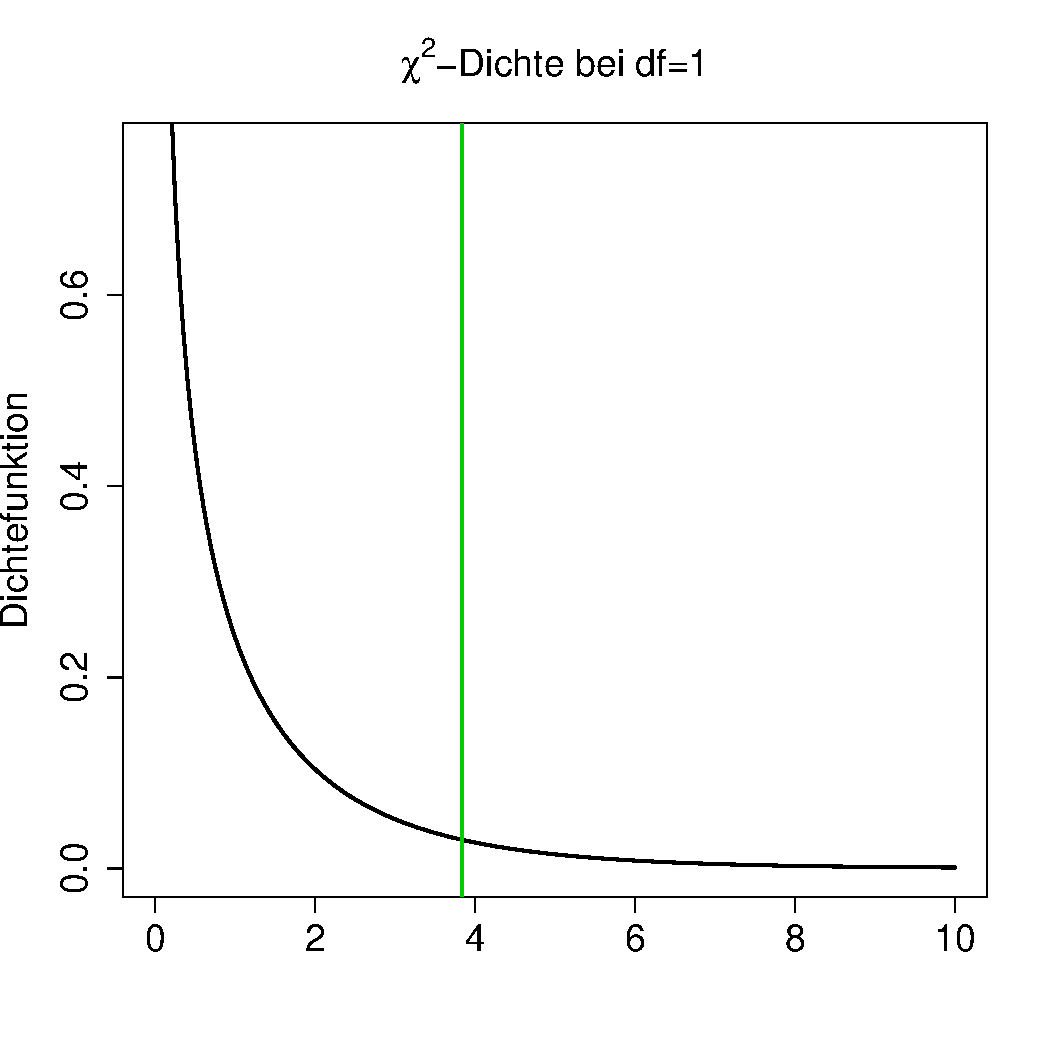
\includegraphics[width=0.85\textwidth]{chi2.pdf}
 	      \caption{Dichte der $\chi^{2}$-Verteilung mit einem Freiheitsgrad
 	       \label{abb1}}
 	\end{figure}
% https://stats.idre.ucla.edu/other/mult-pkg/whatstat/ 	
%http://www.reed.edu/psychology/stata/analyses/nonparametric/bitest.html

%Vidio:
% https://www.youtube.com/watch?v=WvlgEWIS9r8
\aufgabe{Approximativer und exakter Binomialtest}\\
\vspace{0.5cm}
%
%%\url{https://www.stata.com/manuals13/rbitest.pdf}
% http://ssc.wisc.edu/sscc/pubs/sfs/sfs-ttest.htm#paired

Ein Politiker behauptet in einer Pressemitteilung mit Bezug auf den Thüringen-Monitor $2015,$ dass der Anteil der Thüringer Wahlbevölkerung
der angibt weniger als seinen gerechten Anteil zu erhalten mittlerweile auf über $50\%$ gestiegen ist. Er behauptet weiter, dass 
dieser Anteil unter den Arbeitslosen sogar mehr als $60\%$ beträgt.
 Schlagen Sie Ihre Formelsammlung auf
S. 49 auf. Der dort beschriebene Test heißt approximativer Binomialtest.
%
%https://www3.nd.edu/~rwilliam/stats1/OneSample-Stata.pdf
% http://data.library.virginia.edu/stata-basics-create-recode-and-label-variables/
\begin{enumerate}
\item{Berechnen Sie $$\frac{9}{p(1-p)}$$ für $p=0.5$ um zu entscheiden, ob der Test für die Überprüfung
der ersten Behauptung des Politikers geeignet ist.}
\item{Um den Test zu rechnen, muss die Variable 
\texttt{Deprivation} in einer binären Kodierung vorliegen. Erzeugen Sie mit dem \texttt{STATA}-Befehl \\  \texttt{. gen depri01 =.} \\
zunächst eine Variable, die nur fehlende Werte enthält. Mit den Befehlen
\\ \texttt{. replace depri01 = 0 if(Deprivation==2)}\\ und \\ \texttt{. replace depri01 = 1 if(Deprivation==1)}\\ haben Sie eine binäre
erzeugen Sie eine binäre Variable. Überprüfen Sie mit den Befehlen 
\texttt{. tab Deprivation} und \texttt{. tab depri01} ob die neue Variable \texttt{depi01}
die gleiche Häufigkeitsverteilung haben.}
\item{Wie hoch ist in der Stichprobe der Anteil derer, die die Frage nach der Deprivation bejahen?}
\item{Nutzen Sie den Befehl \texttt{. prtest depri01 = 0.5} um die Teststatistik des auf Seite 49 beschriebenen Tests zu rechnen.
Interpretieren Sie das Ergebnis und nehmen Sie Stellung zu der ersten Behauptung des Politikers.}
\item{Wie viele Arbeitslose sind in der Stichprobe? Berechnen Sie $$\frac{9}{p(1-p)}$$ für $p=0.6.$ Ist der approximative
Binomialtest für die Testentscheidung geeignet? }
\item{Als Alternative bei kleinen Stichprobenumfängen gibt es den exakten Binomialtest. Dieser Test kann in \texttt{STATA}
mit Hilfe des Befehls \texttt{bitest} aufgerufen werden. Nutzen Sie den \texttt{STATA}-Befehl \\ \texttt{. bitest depri01 = 0.6 if(EWTS==4)}\\
um mit Hilfe des exakten Tests die Behauptung des Politikers zu überprüfen. Wie hoch ist der Anteil der
Personen, die die Frage nach der Deprivation bejahen unter den Arbeitslosen in der Stichprobe? Ist es beruhend
auf diese Stichprobe sinnvoll davon auszugehen, dass der Anteil der Personen die depriviert
in der Grundgesamtheit sind über $60\%$ liegt? Begründen Sie ihre Antwort.}
\item{Es ist erlaubt, den exakten Test bei großen Stichproben zu verwenden. Umgekehrt ist es problematisch
den approximativen Test bei kleinen Stichproben zu verwenden. Nutzen Sie den exakten Test um die erste
Behauptung des Politikers zu überprüfen und vergleichen Sie das Ergebnis mit dem Ergebnis unter Teilaufgabe d).}
\end{enumerate}



\end{enumerate}
\end{document}
